\documentclass[12pt,a4paper]{article}
\usepackage{pgf}
% \usepackage[condensed,math]{kurier}
% \usepackage[T1]{fontenc}
\usepackage{svg}
\usepackage{tikz}
\usepackage{stanli}
\usepackage{afterpage}
\usepackage{multirow}
\usepackage{subfig}
\usepackage{pgfpages}
\usepackage{listings}
\usepackage{rotating}

%\usepackage{times}


\pgfpagesdeclarelayout{boxed}
{
	\edef\pgfpageoptionborder{0pt}
}
{
	\pgfpagesphysicalpageoptions
	{%
		logical pages=1,%
	}
	\pgfpageslogicalpageoptions{1}
	{
		border code=\pgfsetlinewidth{2pt}\pgfstroke,%
		border shrink=\pgfpageoptionborder,%
		resized width=.9\pgfphysicalwidth,%
		resized height=.9\pgfphysicalheight,%
		center=\pgfpoint{.5\pgfphysicalwidth}{.5\pgfphysicalheight}%
	}%
}

\pgfpagesuselayout{boxed}


% Language setting
% Replace `english' with e.g. `spanish' to change the document language
\usepackage[english]{babel}

% Set page size and margins
% Replace `letterpaper' with `a4paper' for UK/EU standard size
\usepackage[a4paper,top=2cm,bottom=1.5cm,left=1.5cm,right=1.5cm,marginparwidth=1.75cm]{geometry}

% Useful packages
\usepackage{amsmath}
\usepackage{graphicx}
\usepackage[colorlinks=true, allcolors=blue]{hyperref}

\title{}
\author{}
\date{}

\begin{document}
	
	\newcommand{\subf}[2]{%
		{\small\begin{tabular}[t]{@{}c@{}}
				#1\\#2
		\end{tabular}}%
	}
	
	\begin{titlepage}
		\begin{center}
			\vspace*{3cm}
			
			\Huge
			\textbf{Simulation and Models: Report}
			
			\vspace{0.3cm}
			\Huge
			Project 1
			
			\vspace{0.8cm}
			\large
			
			%INSTRUCTED BY: MRS. A.A.S.KAUSHLYA
			
			
			\vspace{0.5cm}
			\LARGE
			
			
			\vspace{1.5cm}
			
			\textbf{}
            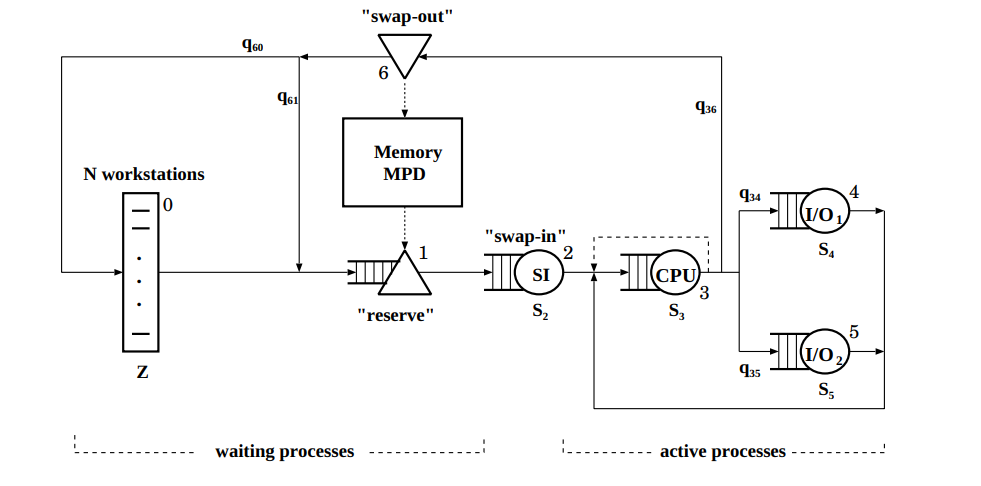
\includegraphics[width=0.8\textwidth]{Images/model.png}
			
			\vfill
			
			
			
			\vspace{0.8cm}
			
			
			
			\Large
			
			
			
			
		\end{center}
		\Large
		\begin{tabbing}
			\hspace*{1em}\= \hspace*{8em} \= \kill % set the tabbings
			\> Name:\>  \textbf{Matteo Ielacqua} \\
			\> ID:\>  \textbf{839241} \\
		\end{tabbing}
		
	\end{titlepage}
	
	
	
	\section{Description of the simulator}
    In this section a brief analysis of the code and other technical aspect of the simulator will be discussed.
    \subsection{Events}
    The simulator is designed to manage a range of events within this system, with a particular focus on two crucial types: the arrival of a client and the departure. Each event type has a distinct impact on the simulator's state, influenced by the specific target under consideration. 
    \begin{itemize}
        \item Departure from the delay station: a departure from the delay station will cause an arrival at the swap-in station.
        \item Arrival to the delay station: an arrival will trigger a departure with a certain delay, that is a Random Variable with a negative exponential distribution of 5000 ms .
        \item Arrival at the Reserve station: if the counter of the process allocated in the system is less than the setted MPD. Then the an arrival event is immediately scheduled for the swap in. Otherwise the information are stored in a queue for later use at the next arrival.
        \item Arrival at the swap in station: an arrival to this station will trigger a departure with a delay, equal to a RV with negative exponential distribution of 210 ms. If at the arrival the station is `occupied' by another client that is waiting it's departure, then the client will be served later with an FCFS policy.
        \item Departure from the swap in station: a departure from the swap in will trigger an immediate arrival to the CPU 
        \item Arrival to the CPU: An arrival to the cpu can be of 2 types, 1) the arrival of a new process has happened, so it is either stored in the ready queue if an another process is under execution or it's executed immediately. In this process a service time with an hyper exponential distribution is assigned to the service. 2) a process that was enqueued in the ready queue is rescheduled for execution , no event under process is expected under this assumption because this type of arrival is accepted only if a departure has appened in the CPU. The exeuction of a process is simulated by scheduling a departure with a delay equal to the time slice of the cpu and subtracting the remaining service time of the process with that time slice.
        \item Departure from the CPU: this event can happen in different conditions which will lead to 2 different behaviour: 1) the process has a remaining service time > 0, so it will be memorized in the ready queue for later use, at this point a new process is Dequeued from the ready queue and scheduled for execution (arrival to the CPU), the actual event under process is resetted. 2) the remaining service time of the process is 0, so an arrival is triggered to the IO1, IO2 or the Swap out with a certain routing probability. A new process is extracted from the ready queue if it is available.
        \item Arrival to IO1/IO2: in both cases an arrival will trigger a departure from the relative station that is an RV with negative exponential distribution.
        \item Departure from IO1/IO2: in both cases this will result in an immediate arrival event to the CPU. 
        \item Arrival to swap out: this event will trigger an immediate departure for the swap out 
        \item Departure from swap out: this event will trigger an immediate arrival to the delay station with p 0.4 or an immediate arrival to the reserve station with p 0.6. In any case this event will decrement by 1 the counter of allocated process in the reserve station.
    \end{itemize}

    \subsection{Choice of the regeneration point}
    Since all the queues follow a markovnian distribution, the regeneration point can be any departure in the system. If we consider all the station that are not the delay as a unique system we can say that the entry point of the processes is the reserve station, and the leave point is the swap out, in any conditions. So we can use a departure from the swap out as a regeneration point, because we expect that the number of clients in the system will be steady after a leave and that a sufficient number of operation will be done by the cpu in order to collect some data.
    \section{First validation step}
    \subsection{Bottleneck analysis}
    In order to start the analysis , let's show here the simplified model 
    used to conduct the validation.
    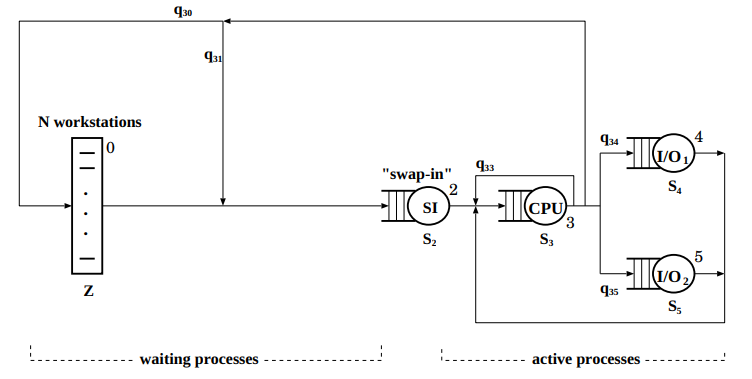
\includegraphics[width=0.8\textwidth]{Images/simplified_model.png}
    \\And summarize some data:
    \begin{displaymath}
        \begin{aligned}
        S_2 = 210ms && S_3= 2.7ms && S_4 = 40ms && S_5=180ms\\
        q_{3,0}= 0.4&& q_{3,1}=0.6 && q_{3,3} = 0.9 && q_{3,4}= 0.065\\
        && q_{3.5}= 0.025 && q_{3,6}=0.01 && 
        \end{aligned}
    \end{displaymath}
    Based on this data, it becomes evident that the provided approximation is plausible. Given a process with a 0.9 probability of returning with a mean service time of 2.7, and considering our original model where clients exhibit a mean service time of 27 ms and a fixed CPU slice time of 2.7 ms, we anticipate that a customer will be rescheduled in the CPU nearly nine additional times following the initial scheduling. \\

    From the previous data we can extract this matrix 
    \begin{displaymath}
        \begin{bmatrix}
            0 && 1 && 0 && 0 && 0 \\
            0 && 0 && 1 && 0 && 0 \\
            0.004 && 0.006 && 0.9 && 0.065 && 0.025 \\
            0 && 0 && 1 && 0 && 0 \\
            0 && 0 && 1 && 0 && 0 \\
        \end{bmatrix}
    \end{displaymath}

    From which we can extract the following system of equations 
    \begin{displaymath}
        \begin{cases}
            V_0=0.004V_3\\
            V_2=V_0+0.006V_3\\
            V_3=V_2+0.9V_3+V_4+V_5\\
            V_4=0.065V_3\\
            V_5= 0.025V_3
        \end{cases}
    \end{displaymath}
    with the additional equation $V_0=1$. Resolving this system lead to the computation 
    all $V_i$ 
    \begin{displaymath}
        \begin{cases}
            V_0=1 \\
            V_3=250\\
            V_2=2.5\\
            V_4=16.25\\
            V_5=6.25
        \end{cases}
    \end{displaymath}

    From this computes $V_i$ is possible to detect which of the station is the bottleneck of the system
    by considering that $VbS_b= \max_i\{V_iS_i\}$, so let's compute all $V_iS_i$ and find 
    the greater one. 

    \begin{displaymath}
        \begin{aligned}
            V_2S_2= 525ms && V_3S_3=675ms && V_4S_4=650ms && V_5S_5= 1125ms
        \end{aligned}
    \end{displaymath}
    from this calculation we can say that $V_bS_b=V_5S_5=1125ms$ and so , station 5 (IO2) is 
    our bottleneck. Let's extract some additional information, as the total cycle time when $N=1$ ,i.e Y(1) 
    \begin{displaymath}
        D=\sum_{i=1}^{N}D_i=\sum_{i=1}^{N}V_iS_i=2975ms
    \end{displaymath}
    Thus we can also calculate the saturation point $N^*$ of this system, after which we can expect
    the total response time will increase. 
    \begin{displaymath}
        N^*=\frac{Y(1)}{V_bS_b}=\frac{D}{V_bS_b}=\frac{2975ms}{1125ms}=2.64
    \end{displaymath}
    \subsection{MVA analysis}
    Starting from the previous matrix is possible to compute various measures using the MVA algorithm for Load Indipendent and Delay stations. In order to compute the visits vector is possible to use the power matrix method.
    \begin{lstlisting}[language=C++]
        
    std::vector<double> 
    powerMatrixMethod(Matrix<double> dtmc, int iterations)
    {
        auto old = dtmc;
        auto res = old;
        for(int i = 0; i < iterations; i++){
            res = old*old;
            old = res;
        }

        std::vector<double> result{};
        for(int i = 0; i < res.Rows(); i++)
            result.push_back(res(i,i));
        return result;
    }
    \end{lstlisting}
    That requires only to multiply the transition matrix for an arbitrary number of iterations, then pick the elements on the diagonal, that are the probability mass flowing in to the i-th station. Let the previously obtained vector be $D$, at this point the visits can be computed with this simple formula $V_i=D_i*\frac{1}{D_0} \ \ \ i=1 \dots N$. In c++ this translate to:
    \begin{lstlisting}[language=C++]
        // compute the visits vector with 
        // 10000 iteration of power matrix method
        std::vector<double> visits = powerMatrixMethod(q, 10000);
        for (int i = 1; i < visits.size(); i++)
        {
            visits[i] = visits[i] * (1 / visits[0]);
        }
    \end{lstlisting}
    At this point is possible to apply the MVA algorithm, that result in subsequent values.
    \\
    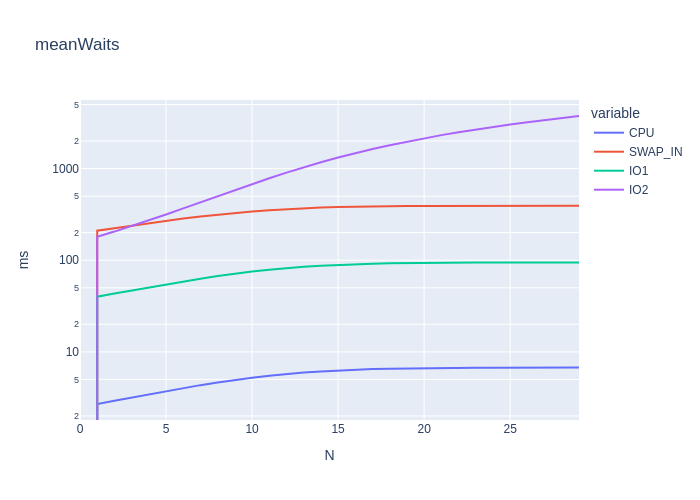
\includegraphics[width=0.9\textwidth]{Images/meanWaits.png}\\
    <da commentare>
    \\
    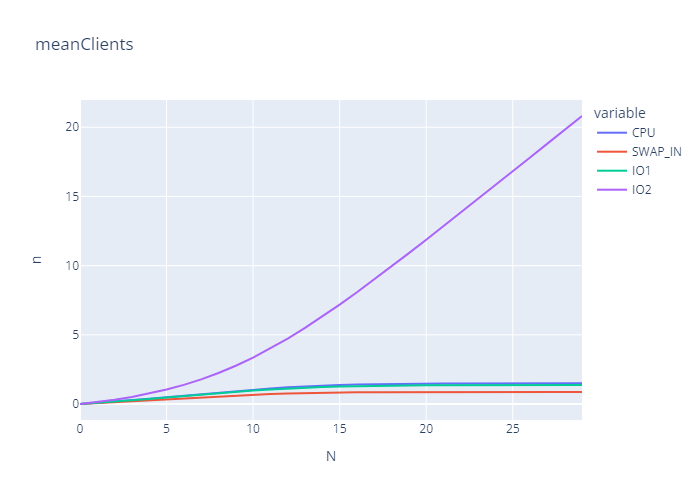
\includegraphics[width=0.9\textwidth]{Images/meanClients.png}
    \\
    <da commentare>
    \\
    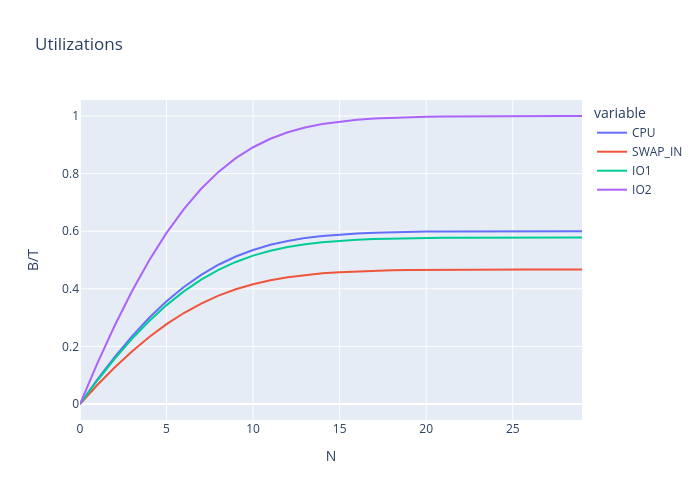
\includegraphics[width=0.9\textwidth]{Images/Utilizations.png}\\
    <da commentare>
    \\
    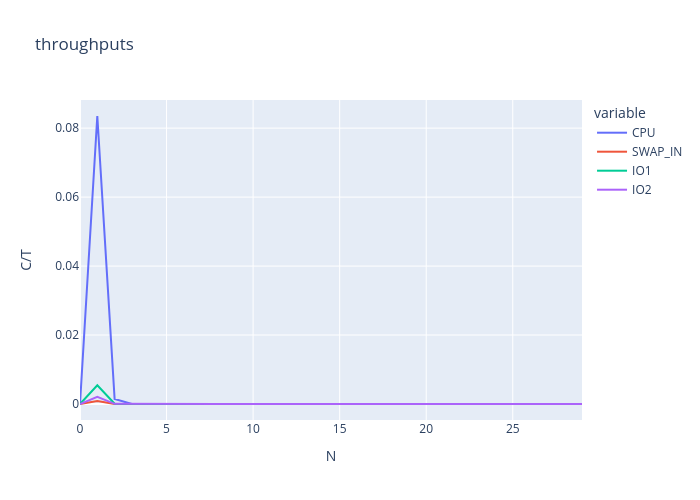
\includegraphics[width=0.9\textwidth]{Images/throughputs.png}
    \\
    <da commentare>
    \\
    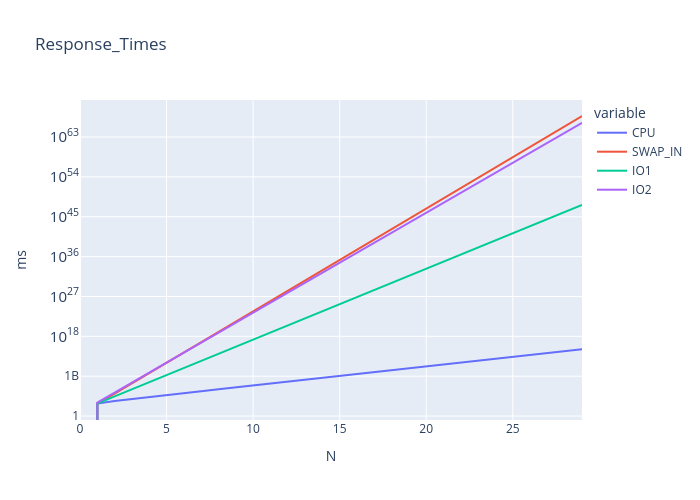
\includegraphics[width=0.9\textwidth]{Images/Response_Times.png}
    \\
    <da commentare>
    \end{document}